\documentclass[10pt,a4paper]{article}
\usepackage[utf8]{inputenc}
\usepackage{polski}
\usepackage{graphicx}
\usepackage{multirow}
\usepackage{longtable}
\usepackage{array}
\usepackage{enumitem}
\usepackage{listings}
\renewcommand\labelenumii{\arabic{enumii}.}
\author{
  \small Mateusz Forc\\
  \small Wiktor Franus\\
  \small Hubert Jatkowski\\
  \small Przemysław Kopański\\
  \small Grzegorz Staniszewski\\
}
\title{Sklep Internetowy}
\begin{document}
  \maketitle
  \begin{abstract}
    \center 
    Aplikacja bazodanowa realizowana na przedmiot \newline 
           Bazy Danych 2 w semestrze 2016Z.
  \end{abstract}
  \tableofcontents
  \newpage
  \section{Projekt Bazy Danych}
  
    \subsection{Diagram ER wraz z opisem związków}
      \begin{center}
        \includegraphics[scale=0.3]{ER}
      \end{center}
          \newpage 
    \subsection{Opis Encji}
     \textbf{Client} - encja reprezentująca klienta
      \begin{center}
        \begin{tabular}{| m{3cm} | m{3cm} | m{3cm} | m{3cm} |}
          \hline
          Nazwa atrybutu & Typ danych & Obligatoryjność & Opis\\ \hline
		  id        & PK INTEGER    & NOT NULL 		    & -\\ \hline
		  name      & STRING        & NOT NULL 			& -\\ \hline
		  surname   & STRING        & NOT NULL 			& -\\ \hline
		  birthdate & DATE          & NOT NULL 			& -\\ \hline
		  address   & TEXT          & NOT NULL 			& -\\ \hline
		  email     & UNIQUE STRING & NOT NULL 			& -\\ \hline
		  login     & UNIQUE STRING & NOT NULL 			& -\\ \hline
		  password  & STRING        & NOT NULL 			& -\\ \hline
		\end{tabular}
	  \end{center}

	  \flushleft \textbf{Employee} - encja reprezentująca pracownika
	  \begin{center}
        \begin{tabular}{| m{3cm} | m{3cm} | m{3cm} | m{3cm} |}
          \hline
          Nazwa atrybutu & Typ danych 	 & Obligatoryjność & Opis\\ \hline
		  id  			 & PK INTEGER 	 & NOT NULL 	   & -\\ \hline
		  name 			 & STRING 	  	 & NOT NULL 	   & -\\ \hline
		  surname 		 & STRING 	  	 & NOT NULL 	   & -\\ \hline
		  pesel 		 & UNIQUE STRING & NOT NULL 	   & -\\ \hline
		  birthdate 	 & DATE 		 & NOT NULL 	   & -\\ \hline
		  address 	  	 & TEXT 		 & NOT NULL 	   & -\\ \hline
		  email 		 & UNIQUE STRING & NOT NULL 	   & -\\ \hline
		  login 		 & UNIQUE STRING & NOT NULL 	   & -\\ \hline
		  password 		 & STRING 		 & NOT NULL 	   & -\\ \hline
		\end{tabular}
	  \end{center}
	  
	  \flushleft \textbf{Review} - encja reprezentująca opinię klienta o towarze
	  \begin{center}
        \begin{tabular}{| m{3cm} | m{3cm} | m{3cm} | m{3cm} |}
          \hline
          Nazwa atrybutu & Typ danych & Obligatoryjność & Opis\\ \hline
		  id 			 & PK INTEGER & NOT NULL 	    & -\\ \hline
		  rating 		 & INTEGER 	  & NOT NULL 		& Ocena produktu w skali od 1 do 5\\ \hline
		  comment 		 & TEXT 	  & NOT NULL 		& Tekst opinii wprowadzony przez autora\\ \hline
		  date 			 & TIMESTAMP  & NOT NULL 		& Data dodania opinii\\ \hline
		  client\_id 	 & FK INTEGER & NOT NULL 		& ID klienta, który dodał opinię\\ \hline
		  item\_id 		 & FK INTEGER & NOT NULL 		& ID produktu, którego dotyczy opinia\\ \hline
		\end{tabular}
	  \end{center}
	
	  \newpage
	  \flushleft \textbf{Order} - encja reprezentująca zamówienie na towary
      \begin{center}
        \begin{tabular}{| m{3cm} | m{3cm} | m{3cm} | m{3cm} |}
          \hline
          Nazwa atrybutu 	   & Typ danych & Obligatoryjność & Opis\\ \hline
		  id 		  	 	   & PK INTEGER & NOT NULL 		  & -\\ \hline
		  date 			 	   & TIMESTAMP  & NOT NULL 		  & Data złożenia zamówienia\\ \hline
		  status 		 	   & INTEGER 	& NOT NULL 		  & Informacja, czy zamówienie jest złożone, 
		  												        w realizacji, czy sfinalizowane\\ \hline
		  status\_change\_date & TIMESTAMP 	& NOT NULL 		  & Data ostatniej zmiany statusu\\ \hline
		  payment\_status 	   & INTEGER 	& NOT NULL 		  & Status płatności za zamówienie\\ \hline
		  client\_id 		   & FK INTEGER & NOT NULL 		  & ID klienta, który złożył zamówienie\\ \hline
		\end{tabular}
	  \end{center}

	  \flushleft \textbf{Item} - encja reprezentująca towar na składzie
      \begin{center}
        \begin{tabular}{| m{3cm} | m{3cm} | m{3cm} |  m{3cm} |}
          \hline
          Nazwa atrybutu & Typ danych & Obligatoryjność & Opis\\ \hline
		  id 			 & PK INTEGER & NOT NULL 		& -\\ \hline
		  name 			 & STRING 	  & NOT NULL 		& Nazwa towaru\\ \hline
		  price 		 & DECIMAL 	  & NOT NULL 		& Cena towaru\\ \hline
		  description 	 & STRING 	  & NOT NULL 		& Dokładniejszy opis towaru\\ \hline
		  in\_stock 	 & INTEGER 	  & NOT NULL 		& Liczba sztuk towaru na składzie\\ \hline
		  category\_id 	 & FK INTEGER & NOT NULL 		& ID kategorii, do której należy towar\\ \hline
		\end{tabular}
	  \end{center}

	  \flushleft \textbf{Order\_Item} - encja pośrednicząca pomiędzy Order i Item
	  \begin{center}
        \begin{tabular}{| m{3cm} | m{3cm} | m{3cm} |  m{3cm} |}
          \hline
          Nazwa atrybutu & Typ danych & Obligatoryjność & Opis\\ \hline
		  id 			 & PK INTEGER & NOT NULL 		& -\\ \hline
		  quantity 	 	 & INTEGER 	  & NOT NULL 		& Liczba sztuk towaru w zamówieniu\\ \hline
		  price 		 & DECIMAL 	  & NOT NULL 		& Cena towaru za sztukę, 
		  							               		  za który został sprzedany w danym zamówieniu\\ \hline
		  order\_id 	 & FK INTEGER & NOT NULL 		& ID zamówienia, do którego należy pozycja\\ \hline
		  item\_id 		 & FK INTEGER & NOT NULL 		& ID towaru, na który wskazuje pozycja\\ \hline
		\end{tabular}
	  \end{center}
	   
	  \newpage
	  \flushleft \textbf{Category} - encja reprezentująca kategorię, do której może należeć towar
      \begin{center}
        \begin{tabular}{| m{3cm} | m{3cm} | m{3cm} |  m{3cm} |}
          \hline
          Nazwa atrybutu & Typ danych & Obligatoryjność & Opis\\ \hline
		  id 			 & PK INTEGER & NOT NULL 		& -\\ \hline
		  name 			 & STRING 	  & NOT NULL 		& Nazwa kategorii\\ \hline
		\end{tabular}
	  \end{center}

	  \flushleft \textbf{Invoice} - encja reprezentująca fakturę
	  \begin{center}
        \begin{tabular}{| m{3cm} | m{3cm} | m{3cm} |  m{3cm} |}
          \hline
          Nazwa atrybutu & Typ danych 	  & Obligatoryjność & Opis\\ \hline
          order\_id 	 & PK FK INTEGER  & NOT NULL 		& ID zamówienia, na które została wystawiona faktura\\ \hline
		  unique\_no 	 & UNIQUE INTEGER & NOT NULL 		& Numer faktury\\ \hline
		\end{tabular}
	  \end{center}
  \newpage
  \section{Projekt Aplikacji}
    \subsection{Słownik pojęć}
        \begin{itemize}
		  \item \textbf{Sklep internetowy} – aplikacja, która jest przedmiotem niniejszego projektu.
		  \item \textbf{Administrator sklepu} - pracownik sklepu zarządzający kontami innych pracowników
          \item \textbf{Klient/Użytkownik anonimowy} – osoba niezarejestrowana w systemie,
           	    		korzystająca z serwisu w celu zakupu towarów.
		  \item \textbf{Klient/Użytkownik zarejestrowany} – osoba zarejestrowana w systemie (posiadająca konto),
		  				korzystająca z serwisu w celu zakupu towarów.
		  \item \textbf{Pracownik sklepu} – użytkownik zarejestrowany zarządzający aplikacją, posiada dostęp do edycji 									towarów, kategorii, zamówień i opinii w sklepie internetowym.
		  \item \textbf{Nazwa użytkownika} – nazwa, którą użytkownik będzie posługiwał i identyfikował się w serwisie,
		  	    		nazwa użytkownika jest niezbędna podczas logowania.
		  \item \textbf{Hasło użytkownika} – ciąg znaków, używany do logowania się do serwisu oraz uzyskiwania dostępu 
		  				do pełnych funkcji serwisu.
		  \item \textbf{Towar} – produkt sprzedawany.
		  \item \textbf{Zamówienie} – lista towarów (wraz z ilością sztuk) wybranych i zatwierdzonych przez 
		  				klienta w celu zakupu.
		  \item \textbf{Opinia} - komentarz słowny i/lub ocena punktowa w skali 1-5 użytkownika zarejestrowanego 
		  				na temat zakupionego towaru
		  \item \textbf{Koszyk} – podręczna lista towarów wybranych przez klienta.
		  \item \textbf{E-faktura VAT} – dokument elektroniczny wystawiany przez czynnych podatników VAT, 
		  				potwierdzający przeprowadzenie czynności podlegającej opodatkowaniu VAT
		  \item \textbf{Przeglądarka internetowa} – program komputerowy służący do pobierania i 
		  	    		wyświetlania stron internetowych udostępnianych przez serwery WWW.
		\end{itemize}
	  \newpage
	  \subsection{Wymagania Funkcjonalne}
	  	\flushleft
          \begin{longtable}{| m{0.5cm} | m{4cm} | p{6cm} | m{1.5cm} |}
            \hline
            Lp. & Nazwa wymagania 						& Opis 										& Priorytet\\ \hline
            \multicolumn{4}{|l|}{Funkcjonalności dostępne bez konieczności logowania}\\ \hline
            1.  & Wyświetlenie listy dostępnych towarów & Wyświetlenie listy zawierającej zdjęcie, 
            											  nazwę i cenę dla każdego towaru.			& 1\\ \hline
            2.  & Wyświetlanie szczegółowych danych na 
            	  temat konkretnego towaru				& Wyświetlanie widoku szczegółowego 
            	  										  zawierającego nazwę, zdjęcie, opis oraz
            	  										  cenę konkretnego towaru.					& 1\\ \hline
			3.  & Wyszukiwanie towarów					& Wyszukiwanie i wyświetlanie listy 
														  towarów o wpisanej nazwie. Powinny zostać 
														  wyświetlone zarówno towary, których nazwa 
														  jest identyczna z wpisaną, jak i te,
														  których nazwa częściowo pokrywa się 
														  ze wpisaną frazą.							& 2\\ \hline
			4.	& Rejestracja nowego klienta w systemie & Rejestracja nowego użytkownika w systemie
														  wymaga podania danych obowiązkowych, tj.:
														  
														  \begin{itemize}[label={--}]
														  \item Imię i nazwisko użytkownika
														  \item Adres e-mail użytkownika
														  \item Nazwa użytkownika
														  \item Hasło użytkownika
														  \item Adres zamieszkania użytkownika
														  \end{itemize}
														  Oraz danych opcjonalnych, tj.:
														  \begin{itemize}[label={--}]
														  \item Adres do wysyłki
														      (jeżeli inny niż adres zamieszkania)
														  \item Datę urodzenia użytkownika.
														  \end{itemize}								& 1\\ \hline
			5. & Logowanie klienta						& Uwierzytelnianie użytkownika za pomocą 
														  nazwy użytkownika i hasła. 
														  Zawartość koszyka nie ulega zmianie 
														  po zalogowaniu.							& 1\\ \hline
														  
			6. & Wyświetlanie informacji 
			     o przedsiębiorstwie prowadzącym 
			     niniejszy sklep internetowy			& Wyświetlanie nazwy, pełnego adresu 
			     										  oraz numeru telefonu przedsiębiorstwa.    & 3\\ \hline
			\multicolumn{4}{|c|}{Funkcjonalności dostępne dla zarejestrowanego użytkownika
			wszystkie powyższe oraz:}\\ \hline
			7. & Edytowanie swoich danych				& Możliwość edycji poniższych danych:
														  \begin{itemize}[label={--}]
														  \item Adresu e-mail użytkownika
														  \item Hasła użytkownika
														  \item Adresu zamieszkania użytkownika
														  \item Adresu do wysyłki.					
														  \end{itemize}								& 2\\ \hline
										  
			8. & Dodawanie towarów do koszyka 			& Dodawanie do koszyka towaru wybranego 
														  przez użytkownika. Ponowne dodanie tego
														  samego towaru do koszyka skutkuje 
														  zwiększeniem ilości sztuk 
														  tego towaru w koszyku.					& 1\\ \hline
														  
			9. & Zmiana ilości sztuk towarów w koszyku & Zmiana ilości sztuk dla wybranego towaru 
														 znajdującego się aktualnie w koszyku. 		& 2\\ \hline
														 
			10.& Usuwanie towarów z koszyka			   & Usuwanie z koszyka towarów wybranych 
														 przez użytkownika. 						& 1\\ \hline
			11.& Składanie zamówienia				   & Składanie zamówienia na towar znajdujący
														 się aktualnie w koszyku. Po złożeniu 
														 zamówienia wyświetlane jest jego 
														 potwierdzenie. Potwierdzenie to jest 
														 również wysyłane na adres e-mail
														 użytkownika, który to zamówienie złożył.   & 1\\ \hline
			12.& Śledzenie statusu zamówienia		   & Wyświetlanie poprzednich oraz aktualnego
														 statusu zamówienia. Wyświetlanie 
														 daty i godziny każdej zmiany statusu. 
														 Zamówienie może mieć w danym momencie 
														 jeden z następujących statusów:
														 \begin{itemize}[label={--}]
														 \item zarejestrowane
														 \item w realizacji
														 \item wysłane
														 \item zrealizowane
														 \item anulowane
														 \end{itemize}								& 2\\ \hline
			13.& Wyświetlanie historii zamówień        & Wyświetlanie chronologicznej listy wszystkich
			 											 zamówień złożonych przez 
			 											 zalogowanego użytkownika						& 1\\ \hline
			 											 
			14.& Zlecenie wystawienia e-faktury VAT    & Możliwość zlecenia wystawienia e-faktury VAT 
														 w momencie składania zamówienia				& 2\\ \hline
			15.& Dodawanie opinii na temat towaru	   & Dodawanie opinii o wybranym produkcie poprzez 
														 napisanie komentarza oraz/lub wybranie 
														 ilości „gwiazdek” w skali 1-5,
														 gdzie 5 oznacza wartość najlepszą.				& 3\\ \hline
			 \multicolumn{4}{|c|}{Funkcjonalności dostępne dla pracownika sklepu
			 					  wszystkie powyższe oraz:}\\ \hline
			16.& Dodawanie towaru					   & Dodawanie nowego towaru do bazy dostępnych
			 											 towarów poprzez podanie jego: nazwy,
			 											 kategorii do której należy, opisu,
			 											 ceny oraz ilości sztuk. 
			 											 Do każdego towaru można dodać zdjęcie. 
			 											 W przypadku nie dodania zdjęcia przez pracownika
			 											 sklepu, system dodaje zdjęcie domyślne.		& 1\\ \hline
			17.& Usuwanie towaru					   & Usuwanie wybranego towaru z bazy.				& 1\\ \hline
			18.& Edytowanie danych towaru			   & Możliwość edycji wszystkich danych powiązanych
														 z wybranym towarem.							& 1\\ \hline
			19.& Dodawanie kategorii				   & Dodawanie kategorii towarów poprzez 
														 podanie jej nazwy i opisu.						& 1\\ \hline
			20.& Usuwanie kategorii					   & Usuwanie wybranej kategorii z bazy.			& 1\\ \hline
			21.& Zmiana statusu zamówienia			   & Zmiana statusu zamówienia na inny. 
														 Dostępne statusy wymieniono w punkcie 12.		& 2\\ \hline
			22.&Usuwanie opinii 					   & Usuwanie z bazy danych opinii wystawionych
														 przez użytkowników								& 3\\ \hline
														 
			\multicolumn{4}{|c|}{Funkcjonalności dostępne dla administratora sklepu}\\ \hline
			23.&Dodawanie pracownika				   & Dodawanie nowego konta pracownika do systemu.
														 Dodanie pracownika wymaga podania identycznych
														 danych jak przy rejestracji klienta
														 z uwzględnieniem poniższych wyjątków:
														 \begin{itemize}[label={--}]
														 \item Data urodzenia jest obowiązkowa
														 \item Wymagane jest również podanie numeru PESEL.  
														 \end{itemize}									& 1\\ \hline
			24.&Usuwanie pracownika					   & Usuwanie wybranego użytkownika z bazy.			& 1\\ \hline
			25.&Edytowanie danych pracownika		   & Możliwość edycji wszystkich danych 
														 wybranego użytkownika.							& 1\\ \hline
     		\multicolumn{4}{|c|}{Pozostałe funkcjonalności}\\ \hline
			26.&Generowanie e-faktur VAT			   & Generowanie e-faktur VAT za zamówienia,
														 dla których zostały wysłane zlecenia 
														 wystawienia e-faktury VAT						& 2\\ \hline
			27.&Wysyłanie e-faktur do klienta
			    zarejestrowanego					   & Wysyłanie wygenerowanych e-faktur na 
			    										 adres e-mail klienta, który złożył 
			    										 zlecenie wygenerowania e-faktury 
			    										 dla konkretnego zamówienia.					& 2\\ \hline


    \end{longtable}
    \newpage
    \subsection{Wymagania niefunkcjonalne:}
      \begin{enumerate}
	    \item Dostęp do sklepu internetowego przez 24h na dobę.
	    \item Dostęp do sklepu internetowego za pomocą przeglądarki internetowej.
		\item W celu złożenia zamówienia konieczna jest rejestracja oraz zalogowanie w systemie.
		\item Każdy użytkownik ma ograniczone prawa dostępu do systemu.
		\item Konto każdego użytkownika chronione jest nazwą użytkownika i hasłem. Hasło nie może być przechowywane w bazie 				  danych w formie jawnej. Jest zaszyfrowane funkcją skrótu.
		\item System powinien obsługiwać około 10 000 towarów.
		\item System powinien obsługiwać około 100 000 zarejestrowanych użytkowników.
		\item System powinien obsługiwać około 100 jednocześnie połączonych użytkowników.
		\item E-faktury VAT generowane przez sklep internetowy muszą spełniać wszystkie wymogi 
			  polskiego prawa dotyczące e-faktur. 
	   \end{enumerate}
	  \newpage
      \subsection{Schemat logiczny}
        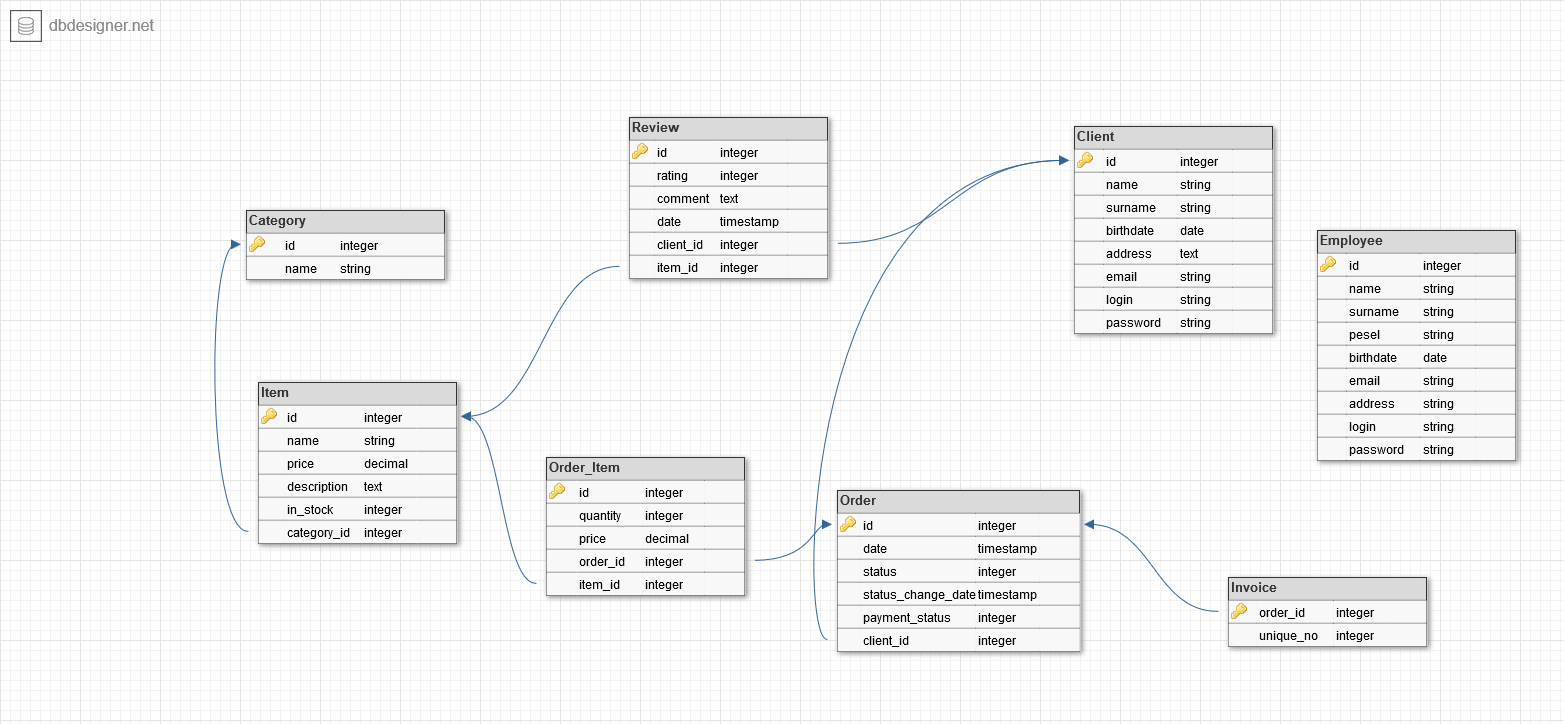
\includegraphics[scale=0.2]{schematlogiczny}
      \newpage
      \subsection{Skrypt DDL tworzący bazę danych}
		\lstinputlisting[language=SQL]{DDL_schema.sql} 
\end{document}